\chapter{Results and Evaluation}
\label{ch:results}

% Tables under tables/ are generated by `python -m src.analysis.report` from outputs/ and committed.
% The \IfFileExists guards let the dissertation build whether or not they have been generated yet.

This chapter reports what the measurements show. It opens by checking that the frozen tracker reproduces the
published benchmark. It then works through the model in the order the decision rule of
Section~\ref{sec:meth-success} demands: the fitted coefficients, how much variance the distances explain
together with the intrinsic-difficulty pivot, and the out-of-sample test that settles the research question.
Further sections cover the species hold-out, false positives on hard negatives, the robustness variants and
the familiarity proxy. The last three take the analysis to a second dataset, draw the cross-dataset synthesis,
and substitute two other trackers. Supporting tables numbered B.* are collected in
Appendix~\ref{app:supplementary}.

\section{Measurement}
\label{sec:measurement}
Before any modelling, the measurement itself has to be sound. Zero-shot SAM\,3 on the SA-FARI test split
reproduces the published benchmark: the dataset-level (micro) \texttt{VEval} score is $\approx\!0.65$
mask-\texttt{pHOTA}, matching the operating point reported with the dataset.

Table~\ref{tab:gate1} reports a different and lower quantity. It gives the three mask metrics --- detection,
association, and their combination --- as support-weighted means over the $346$ positive cells, which is the
form the model is fitted on. Detection, the primary target, sits at $0.527$, and combined \texttt{pHOTA} at
$0.533$. The gap from $0.65$ is not a discrepancy. The micro figure pools every frame in the dataset into a
single score, whereas this one averages within each cell first and counts positive cells only
(Section~\ref{sec:meth-measure}).
\IfFileExists{tables/gate1_measurement.tex}{% generated by src/analysis/report.py --- do not edit by hand
\begin{table}[htbp]\centering
  \caption{Zero-shot SAM\,3 on the SA-FARI test split --- support-weighted mean over 346 scored cells (of 1447).}
  \label{tab:gate1}
  \begin{tabular}{lr}
    \toprule
    Metric (mask) & Value \\
    \midrule
    pDetA & 0.527 \\
    pAssA & 0.546 \\
    pHOTA & 0.533 \\
    \bottomrule
  \end{tabular}
\end{table}
}{}

\section{Fitted coefficients}
\label{sec:coefficients}
This section reports the first of the two criteria a distance must clear (Section~\ref{sec:meth-success}): does
its coefficient's confidence interval exclude zero? Table~\ref{tab:coefficients} answers that for the location
split, Split~B, over the same $346$ positive cells as Table~\ref{tab:gate1}. The species hold-out is reported
separately in Section~\ref{sec:species-holdout}.

Each row of the table is one factor, and the two columns give its coefficient and confidence interval for
detection and for association. Three features of its construction should be noted.

The coefficients are standardised. Each is the change in the logit of the score for a one-standard-deviation
rise in that factor. Magnitudes can therefore be compared down a column, even though the raw factors are in
quite different units: tree steps, cosine gaps, a binary flag. A negative coefficient means the score falls
as the factor rises, which is the direction H1 and H2 predict.

The intervals are not the model's own. A distance is constant within a species or a location, so the $346$
cells behave like only a few tens of independent groups. These intervals resample whole species and whole
locations instead (Section~\ref{sec:meth-inference}). They are wide deliberately, and that width is the real
uncertainty rather than a defect of the data.

Only three of the four distances appear. Temporal gap is absent because it carries no variance to estimate
from and the model drops it (Section~\ref{sec:meth-temporal}). The last two rows are a scene covariate and the
support control rather than distances.

On this reading, no factor satisfies criterion~(i). Every interval spans zero, for detection and
association alike. Criterion~(i) already fails, before the out-of-sample test of Section~\ref{sec:headline} is
reached.

Two further details are relevant. First, the point estimates for taxonomic and visual distance are negative
here, nominally the direction H1 predicts. The intervals are, however, far too wide for that sign to carry
information, and on the species hold-out, where species novelty actually varies, both coefficients are
positive (Section~\ref{sec:species-holdout}), the opposite of what H1 predicts.

Second, taxonomic distance carries by far the widest interval, $[-3.87,+0.09]$ for detection. That is a
property of this split rather than a finding about taxonomy. The official split shares species across train and
test, so taxonomic distance is $\approx\!0$ for almost every cell here, and the coefficient is estimated from
almost no variation. It is measured imprecisely rather than measured and refuted, and is counted as neither.
The constructed species hold-out is designed to test species novelty properly.
\IfFileExists{tables/coefficients.tex}{% generated by src/analysis/report.py --- do not edit by hand
\begin{table}[t]\centering
  \caption{Standardised logit-GLM coefficients (95\% CI) for detection (pDetA) and association (pAssA).}
  \label{tab:coefficients}
  \begin{tabular}{lcc}
    \toprule
    Factor & pDetA coef.\ [CI] & pAssA coef.\ [CI] \\
    \midrule
    Taxonomic distance & -0.362 [-0.41, -0.32] & -0.368 [-0.41, -0.32] \\
    Temporal gap & -0.000 [-0.00, -0.00] & -0.000 [-0.00, -0.00] \\
    Visual distance & -0.144 [-0.17, -0.12] & -0.122 [-0.14, -0.10] \\
    Environment distance & 0.042 [0.02, 0.06] & 0.013 [-0.01, 0.03] \\
    Clutter & -0.066 [-0.09, -0.04] & -0.087 [-0.11, -0.06] \\
    Night / IR & -0.405 [-0.45, -0.36] & -0.462 [-0.51, -0.41] \\
    log(support) & -0.216 [-0.24, -0.20] & -0.224 [-0.24, -0.20] \\
    \bottomrule
  \end{tabular}
\end{table}
}{}

\section{How much the distances explain, and the difficulty pivot}
\label{sec:variance-difficulty}
The first question is how much of the variation in detection the four distances account for. They account
for almost none of it. A dominance analysis puts the four together at only $\approx 3\%$ of the variation, and no single
distance stands out (Table~\ref{tab:variance}). The method is LMG/Shapley, which splits shared explanatory
power fairly between correlated predictors rather than double-counting it.

One possible explanation is that the distances are so correlated with one another that a real effect cancels out
between them. The VIF column rules that out. The variance inflation factor measures how entangled each
predictor is with the others, and a value near $1$ means essentially independent. Every VIF here is
$\approx 1$, so the $3\%$ is the total explanatory contribution rather than a signal masked by collinearity.


The only distance with an apparent predictive relationship was visual distance, and that relationship is
attributable to animal size. Visually distinctive species tend to be larger, and larger animals are easier to
detect. The apparent novelty effect is therefore confounded with size.

A complementary question follows: whether the intrinsic difficulty of the scene, rather than the novelty of
the animal, predicts detection. Three label-free scene properties are tested against the same criteria: low
light, visual clutter, and a night/IR flag (Table~\ref{tab:difficulty}, Appendix~\ref{app:supplementary}).
Each is measured directly from the frames, with no SAM\,3 run and no target label.

Combined with animal size, these difficulty signals improve on the baseline by $+0.017$ and $+0.020$ on the
two hold-outs. Separating the contributions shows that the entire gain comes from size. Size \emph{on its
own} accounts for it. Low light \emph{on its own} does not improve on the baseline, and adds almost nothing
once size is accounted for.

The apparent night/IR effect is inflated by being measured at the wrong level. Per location, its correlation
with detection looks moderate, at $r=-0.377$. That is an averaging artefact. Measured at the level of the
individual cell, where the model actually operates, it shrinks to $-0.13$, and clutter's is $0.00$. The
intrinsic-difficulty hypothesis is therefore \textbf{also null}: the only label-free property that predicts
detection is animal size.


\section{The primary out-of-sample test: predicting unseen species and locations}
\label{sec:headline}
This is the primary test. The model is fitted on a subset of species and locations, then used to predict
detection for held-out species and locations excluded from fitting. Its error is compared against the
simplest baseline: predicting the mean score in every case.

Table~\ref{tab:cv} reports that comparison. Each row is one combination of hold-out scheme and target, so the
four rows cover leave-species-out and leave-location-out for both detection and association, all within the
same $346$ positive cells. The MAE column is the model's mean absolute error, and Baseline is the mean
predictor's. $\Delta$ is the gain of one over the other, so a positive value indicates lower error than the
mean predictor. The interval comes from the paired group-bootstrap, and the $p$-value is one-sided
(Section~\ref{sec:meth-cv}).

The result is a \textbf{null}. Every gain falls between $+0.004$ and $+0.007$, every interval spans zero, and
no $p$-value drops below $0.13$. On both hold-out schemes, and for both targets, the distance model does not
improve on the mean predictor.

Figure~\ref{fig:predvsactual} presents this graphically. Each point is one held-out cell, with its true
detection score on the horizontal axis and the model's out-of-sample prediction on the vertical. A model that
predicted well would place its points along the dashed diagonal. A model that ignored its inputs and returned
the average every time would place them along the horizontal line. The points follow the horizontal line:
the prediction varies negligibly with the true score.

The null is credible because the procedure demonstrably has power. Run unchanged on the same cells, it
\emph{does} recover a real effect. Animal size improves on the baseline out of sample at the identical
criteria, significantly on both schemes ($\Delta\mathrm{MAE}=+0.015$ leave-species-out, $+0.017$
leave-location-out; Table~\ref{tab:difficulty}). A procedure that detects the size effect while returning no
gain for the distances indicates that the distances carry \emph{no} predictive signal: the null result
reflects an absence of signal, and the size result confirms the power to detect one.
\IfFileExists{tables/cv_validation.tex}{% generated by src/analysis/report.py --- do not edit by hand
\begin{table}[htbp]\centering
  \caption[Out-of-sample validation, location split]{Out-of-sample error vs a mean predictor on the \textbf{location split} (Split~B; the $346$ positive
  cells). Each row is one cross-validation grouping scheme --- leave-species-out or leave-location-out ---
  applied within these same cells; $\Delta$ is the MAE gain over baseline, with a paired-bootstrap 95\% CI and
  one-sided $p$. No scheme's gain is significant.}
  \label{tab:cv}
  \begin{tabular}{llrrrcr}
    \toprule
    CV scheme & Target & $n$ & MAE & Baseline & $\Delta$~[95\% CI] & $p$ \\
    \midrule
    location & pAssA & 346 & 0.289 & 0.295 & +0.007~[-0.005,\,+0.018] & 0.13 \\
    location & pDetA & 346 & 0.293 & 0.298 & +0.004~[-0.007,\,+0.015] & 0.23 \\
    species & pAssA & 346 & 0.289 & 0.295 & +0.006~[-0.006,\,+0.017] & 0.16 \\
    species & pDetA & 346 & 0.293 & 0.298 & +0.004~[-0.006,\,+0.015] & 0.24 \\
    \bottomrule
  \end{tabular}
\end{table}
}{}
\begin{figure}[htbp]
\centering
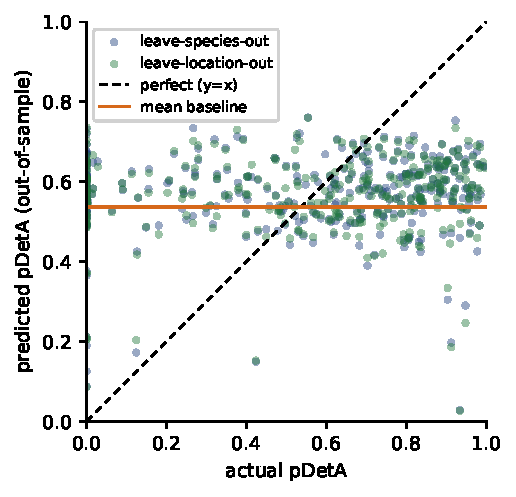
\includegraphics[width=0.44\textwidth]{figures/res_pred_vs_actual.pdf}
\caption[Out-of-sample predicted vs actual]{Out-of-sample detection predictions against the truth, for held-out
species (navy) and held-out locations (green); each point is one cell. Perfect prediction would lie on the
dashed diagonal, and predicting the mean regardless of input lies on the orange horizontal. The points follow
the orange line, so the distances carry no predictive power.}
\label{fig:predvsactual}
\end{figure}

\section{Species hold-out (H1): novelty and the size confound}
\label{sec:species-holdout}
The primary novelty test is a leave-species-out analysis over the pooled train and test species: $99$
species and $1{,}025$ scored cells. Three tables report it, each the Split~A counterpart of one already seen
for Split~B. Table~\ref{tab:gate1_species} (Appendix~\ref{app:supplementary}) gives the measurement, and
confirms the tracker scores in the same range on the pooled set as on the test split alone.
Table~\ref{tab:coefficients_species}, in this chapter, gives the fitted coefficients, and
Table~\ref{tab:cv_species}, also in the appendix, the out-of-sample test.

Out-of-sample prediction again fails. Every gain in Table~\ref{tab:cv_species} is zero or negative, so the
distance model is no better than the mean predictor, and on the species scheme slightly worse.

Table~\ref{tab:coefficients_species} is where this split differs from Split~B. One coefficient does have an interval excluding zero: visual distance, at $+0.37$ for detection. Its sign,
though, is \emph{positive}. Taken at face value, this indicates that more-novel species are detected better,
which is the reverse of what H1 predicts.

It is a \textbf{confound} rather than a reversal. Visually distinctive species tend to be larger
(visual~$\leftrightarrow$~$\log$-area $r=0.22$), and larger animals score higher
($\log$-area~$\leftrightarrow$~\texttt{pDetA} $r=0.30$, the strongest raw correlate of the score). Adding an
animal-size covariate shrinks the visual coefficient from $+0.37$ to $+0.22$, and its interval now spans zero,
while size itself becomes the significant driver. The apparent visual-novelty effect is therefore a size
effect. Taxonomic novelty shows no relationship ($r\approx0.00$).

Figure~\ref{fig:size} shows the same relationship on the location split, where its cell-level correlation is
$r=+0.31$. Each point is one cell, with animal size on the horizontal axis and its detection score on the
vertical. Novelty does not predict transfer; animal size does, weakly.
\begin{figure}[htbp]
\centering
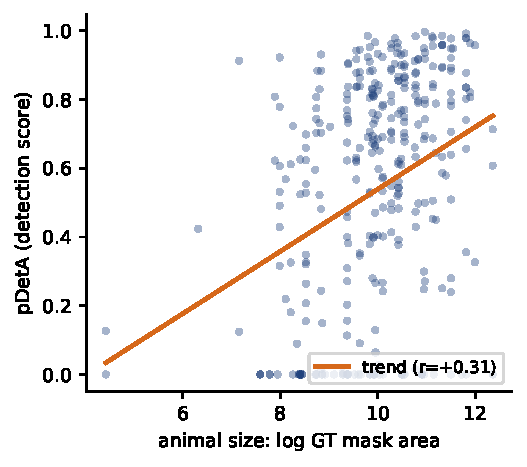
\includegraphics[width=0.44\textwidth]{figures/res_size_confound.pdf}
\caption[The size confound]{The one label-free property that predicts detection: animal size. Per-cell
detection score against log ground-truth mask area, on the location split ($346$ cells), with the fitted trend
at $r=+0.31$. This is the confound behind the apparent visual-distance effect.}
\label{fig:size}
\end{figure}


\IfFileExists{tables/coefficients_species.tex}{% generated by src/analysis/report.py --- do not edit by hand
\begin{table}[htbp]\centering
  \caption{Standardised logit-GLM coefficients with \emph{group-cluster-bootstrap} 95\% CIs (resampling whole species / locations, so the interval respects pseudo-replication and the support weighting), for detection (pDetA) and association (pAssA).}
  \label{tab:coefficients_species}
  \begin{tabular}{lcc}
    \toprule
    Factor & pDetA coef.\ [CI] & pAssA coef.\ [CI] \\
    \midrule
    Taxonomic distance & 0.202 [-0.09, 0.43] & 0.209 [-0.06, 0.42] \\
    Visual distance & 0.369 [0.11, 0.67] & 0.271 [0.04, 0.54] \\
    Environment distance & 0.043 [-0.15, 0.17] & 0.023 [-0.15, 0.13] \\
    Clutter & -0.284 [-0.52, 0.02] & -0.230 [-0.46, 0.06] \\
    Night / IR & -0.286 [-0.77, 0.22] & -0.439 [-0.92, 0.06] \\
    log(support) & -0.020 [-0.14, 0.16] & 0.051 [-0.06, 0.23] \\
    \bottomrule
  \end{tabular}
\end{table}
}{}

\section{False positives / hallucination}
\label{sec:fp}
Everything so far has concerned misses: whether the tracker finds the animals that are there. The detection
score conditions on the animal being present, so it measures recall and is uninformative about hallucination.
The opposite failure (reporting an animal that is not there) is measured on the $1{,}486$ hard negatives, the
queries naming a species absent from the clip. A correct run returns nothing. SAM\,3 nonetheless returns a
masklet in approximately $9.8\%$ of cases.

Table~\ref{tab:fp} asks whether that rate is predictable from the same label-free distances. Each row is one
species-level test, giving the statistic, its $95\%$ confidence interval, and the verdict. The first four rows
are correlations between a species' hallucination rate and one property. The last row is the out-of-sample
test, where the statistic is an MAE gain over a mean predictor rather than a correlation.

This is the closest the study comes to a validated before-running signal. Taxonomic novelty shows no
relationship ($r\approx+0.06$, not significant). Visual distinctiveness does: the more distinctive a species
looks, the \emph{less} the model hallucinates it ($r\approx-0.33$). The relationship remains under an
animal-size control, strengthening to a partial $-0.37$, and size on its own is not significant. Unlike every
earlier effect, this one is not attributable to animal size.

It remains a correlate rather than a predictor. Predicting a held-out species' hallucination rate from visual
distance improves on a mean predictor by only $+0.008$ MAE and does not reach out-of-sample significance
($p=0.053$). Even the strongest signal in the study fails the criterion. Its direction is also the opposite of
the hypothesis: greater distinctiveness is associated with fewer false positives, rather than greater novelty
with worse performance.

\IfFileExists{tables/false_positives.tex}{% generated by src/analysis/report.py --- do not edit by hand
\begin{table}[htbp]\centering
  \caption{False positives on the 1486 hard negatives (113 species): the overall hallucination rate is 9.8\%. More visually distinctive species hallucinate \emph{less} --- a real, size-independent correlate --- but it does not validate out of sample (leave-species-out $p=0.053$), so it is a correlate, not a predictor.}
  \label{tab:fp}
  \begin{tabular}{lccc}
    \toprule
    Test (species-level) & statistic & 95\% CI & verdict \\
    \midrule
    FP rate vs taxonomic distance & $+0.06$ & $[-0.17,\,+0.23]$ & n.s. \\
    FP rate vs \textbf{visual distance} & $-0.33$ & $[-0.43,\,-0.23]$ & significant \\
    \quad visual, size-controlled (partial) & $-0.37$ & $[-0.47,\,-0.28]$ & significant \\
    FP rate vs animal size & $+0.13$ & $[-0.06,\,+0.31]$ & n.s. \\
    leave-species-out OOS gain & $+0.008$ & $[-0.002,\,+0.017]$ & $p=0.053$ \\
    \bottomrule
  \end{tabular}
\end{table}
}{}

\section{Ablations and robustness}
\label{sec:robustness}
The null of Section~\ref{sec:headline} rests on one particular model, built from one particular set of design
choices. This section asks whether either could be responsible for it. The first subsection varies which
factors enter the model. The second holds the factors fixed and varies how they are computed.

\subsection{Factor ablation}
Table~\ref{tab:ablation} (Appendix~\ref{app:supplementary}) refits detection with one change to the design
per row. The pseudo-$R^2$ column is McFadden's, a measure of in-sample fit. The last two columns give the
out-of-sample MAE gain over a mean predictor under the two hold-out schemes, leave-species-out and leave-location-out, each with its $p$-value.

Removing any single distance changes either quantity only marginally, so no single distance carries signal
that the others obscure. Dropping temporal gap changes nothing at all, which is expected: it has no variance and the
model already discards it (Section~\ref{sec:meth-temporal}). Removing the support covariate leaves the model
slightly worse than the baseline ($-0.002$ and $-0.003$), so the null is not that control suppressing a real
effect.

One row does change substantially. Adding the animal-size covariate more than doubles the fit, from $0.055$
to $0.119$, and lifts the out-of-sample gain to significance on both schemes, at $+0.018$ ($p=0.02$) and
$+0.020$ ($p=0.00$) for the full model with the distances included. This is consistent with the variance
partition (Table~\ref{tab:variance}), in which the distances together explain almost nothing.

\subsection{Design robustness}
Table~\ref{tab:robustness} (Appendix~\ref{app:supplementary}) keeps the factor set fixed and swaps a single
design choice per row. Each entry is the out-of-sample gain with its confidence interval and $p$-value, under both hold-out schemes, judged after a
Bonferroni correction over the five variants.

Three swaps test the distances themselves. They change the encoder from DINOv2 to CLIP, take a whole-frame
embedding that keeps the background instead of a mask crop, and replace the nearest-prototype distance with a
distributional Fr\'echet or MMD distance. All leave the gain indistinguishable from the baseline. Every
$\Delta\mathrm{MAE}$ is at most $0.007$, every $p$-value at least $0.10$, and every interval spans zero.

The generic ``animal'' prompt is included for completeness, and produces a different outcome. Prompting
non-specifically collapses per-species detection to a near-constant, mostly-zero target: mean
\texttt{pDetA}$\approx0.14$, with $73\%$ of cells exactly zero. Fitting a target that degenerate, the model
does not merely fail to improve on the mean predictor but falls far below it ($\Delta\mathrm{MAE}\approx-0.35$).

Across every variant the label-free distances fail identically. The null is a property of the transfer
problem, not of one modelling choice.

\section{SAM\,3 familiarity proxy}
\label{sec:familiarity}
Every distance so far has measured novelty against the SA-FARI reference. One objection follows: SA-FARI is
not SAM\,3's training set, and the actual pretraining data is undisclosed, so the distances may fail only
because novelty is measured from the wrong anchor.

The familiarity proxy (Section~\ref{sec:meth-familiarity}) tests that objection by reading familiarity from
SAM\,3 itself, from how separable each species is in its own vision-encoder feature space.
Table~\ref{tab:familiarity} (Appendix~\ref{app:supplementary}) reports the three separability metrics over
the $346$ positive cells. The first two
columns give each metric's out-of-sample gain and $p$-value, on SA-FARI and on BURST. The next two give its
correlation with the DINOv2 visual distance and with animal size, which together show what the metric is really
measuring. The last column is the verdict against a Bonferroni threshold of $\alpha=0.017$ for three metrics.

The result is a further null. None of the three satisfies the criterion on the leave-species-out novelty
test. The strongest, silhouette, reaches only $p=0.034$ for a gain of $+0.012$, and nearest-prototype and
Mahalanobis are further from the threshold, at $p=0.068$ and $0.085$. The null replicates on BURST, where the same three give $p=0.020$,
$0.136$ and $0.148$.

The $r_\text{vis}$ column explains why. All three correlate with the DINOv2 visual distance they re-encode, at
$0.63$ to $0.85$. They largely restate a feature already shown to be null, and in direct comparison none adds
out-of-sample gain over the visual distance plus size. One row differs: silhouette, unlike the
visual distance, is \emph{not} a size artefact ($r_\text{size}=-0.16$). It isolates the size-independent half of
visual distinctness, and still fails to predict transfer.

The metrics do reach significance under leave-location-out ($p\le0.01$), but that is not a novelty test. A
familiarity value is constant within a species, with zero within-species variance. On the location split the
held-out locations' species also appear in training, so a species-constant feature is never tested on an unseen
species at all.

Nor is the null a power failure. On these same $346$ cells the animal-size control does validate out of
sample (Table~\ref{tab:ablation}), so a test returning no gain here reflects an absence of signal rather than
insufficient sensitivity. Reading familiarity from SAM\,3's own representations therefore does not recover
before-running prediction. It restates the same size-entangled visual distinctness that was already null, and
it closes the objection that SAM\,3's true training set is unknown.

\section{Independent replication on a second dataset}
\label{sec:burst}
Both SA-FARI experiments overlay different splits on one frozen inference pass, so they are near-orthogonal
rather than independent (Section~\ref{sec:meth-replication}). BURST~\cite{burst} supplies the independent test:
$132$ cells across $41$ species, mask-native, in a quite different regime of internet, driving and film video
rather than camera traps.

Two preconditions hold there. Zero-shot SAM\,3 is non-degenerate, at \texttt{pHOTA} $0.635$
(Table~\ref{tab:gate1_burst}, Appendix~\ref{app:supplementary}), so there is real variance to model. And the
association target is genuine rather than near-degenerate as it is on SA-FARI: \texttt{pDetA} and
\texttt{pAssA} correlate at $0.76$, and none of the $71$ multi-object cells has them exactly equal. Both components are therefore testable.

Table~\ref{tab:replication_burst} (Appendix~\ref{app:supplementary}) reports the outcome under
leave-species-out cross-validation. Each row is one
predictor, with its out-of-sample MAE gain, confidence interval and $p$-value. The last row is the animal-size
control rather than a distance.

The distances are again null. Combined, they improve out-of-sample error by only $+0.002$ ($p=0.374$), and
individually visual ($+0.003$), taxonomic ($-0.006$) and environment ($-0.001$) are all null. So are the
association specifications. The result survives dropping the $19$ single-cell species, and survives a size
control.

The only near-signal is the same artefact identified above. Visual distance correlates with detection at
$+0.17$ per cell, and at $+0.37$ between species, the same aggregation inflation seen for night/IR in
Section~\ref{sec:variance-difficulty}. Both are \emph{positive}, meaning more-novel animals are detected
better, which is the opposite of the novelty hypothesis. The correlation is also not robust to a size control
(partial $+0.08$, $p=0.35$).

This is a second convergent null rather than positive proof. No before-running quantity reaches significance
here, not even the animal-size control that does validate on SA-FARI. Without a positive control that
reaches significance, the test cannot establish that it would have detected a small species-level effect. What BURST establishes is that no
moderate-or-large before-running distance signal exists in an independent mask-native regime with a genuine
association target. A small species-constant effect cannot be excluded.

\section{Cross-dataset synthesis}
\label{sec:cross_dataset}
Table~\ref{tab:cross_dataset} collects every feature tested, its result on each dataset, and the verdict. The
two dataset columns are not in the same metric, and each header says which it is. BURST entries are
out-of-sample $\Delta$MAE with a $p$-value. SA-FARI entries are standardised GLM coefficients with
confidence intervals, except the rows marked $\dagger$, which are $\Delta$MAE like BURST; the temporal and
hallucination rows report the quantities stated in place. A feature predicts transfer only if it is positive
\emph{and} significant.

The pattern is consistent. No before-running label-free distance, alone or combined, predicts detection or
association transfer out of sample on either dataset, and every gain over a mean predictor sits within
bootstrap noise of zero.

The only near-signal is visual distance, and its direction is the reverse of that predicted: more-novel
animals are detected better, not worse. It does not remain significant under an animal-size control wherever
it is examined.

One row does clear the bar, and it is the confound rather than a hypothesis variable. Animal size validates out
of sample on SA-FARI, modestly. That row doubles as the positive control: the same test that returns no gain
for every distance does detect size, so the null is an absence of signal rather than an absence of power.

The contribution is that null, with its bounds stated and quantified. It is consistent across a camera-trap
dataset and an internet-video one. The clustered intervals cap the visual and environment coefficients at
moderate size, and a planted-effect analysis (Table~\ref{tab:mde}, Appendix~\ref{app:supplementary}) shows
the out-of-sample test reaches $80\%$ power only for standardised effects of $1.5$ (location scheme) to
$1.75$ (species scheme), a gain of $\Delta\mathrm{MAE}\approx+0.02$. Criterion~(ii) therefore certifies the
absence of usable predictive value; effects far smaller than that threshold, including any of the observed
coefficient magnitudes, are bounded by the intervals rather than by the out-of-sample test.
\IfFileExists{tables/cross_dataset_comparison.tex}{% Cross-dataset feature comparison --- hand-maintained; 
\begin{table}[htbp]\centering
  \caption[Cross-dataset synthesis]{Cross-dataset synthesis: every feature tested, per dataset. BURST entries are out-of-sample
  $\Delta$MAE\,($p$); SA-FARI entries are GLM coefficients [95\% CI], except the $\dagger$ rows, which are
  $\Delta$MAE\,($p$) from the species hold-out; the temporal and hallucination rows report the quantities stated in place. Only animal size satisfies the criteria, and only on SA-FARI.}
  \label{tab:cross_dataset}
  \footnotesize
  \setlength{\tabcolsep}{5pt}
  \begin{tabular}{>{\raggedright\arraybackslash}p{3.0cm}ll>{\raggedright\arraybackslash}p{2.8cm}}
    \toprule
    Feature & SA-FARI (coef.\ [CI]) & BURST ($\Delta$MAE, $p$) & Verdict \\
    \midrule
    \multicolumn{4}{l}{\emph{Before-running label-free distances (the research question)}} \\
    Combined distances$^\dagger$ & $-0.004$ ($0.74$)          & $+0.002$ ($0.37$) & null on both \\
    Visual alone                 & $-0.14$ [$-0.50$,\,$0.14$] & $+0.003$ ($0.26$) & null; wrong direction \\
    Taxonomic alone              & $-0.36$ [$-3.87$,\,$0.09$] & $-0.006$ ($0.95$) & null on both \\
    Environment alone            & $+0.04$ [$-0.19$,\,$0.24$] & $-0.001$ ($0.75$) & null on both \\
    Temporal gap                 & $32/1447$, all $=0$        & no timestamps     & untested \\
    \midrule
    \multicolumn{4}{l}{\emph{Confound control}} \\
    Animal size ($\log$-area)$^\dagger$ & $+0.015$ ($0.01$) & $+0.005$ ($0.14$) & \textbf{validates} (SA-FARI) \\
    \midrule
    \multicolumn{4}{l}{\emph{Detection precision (hard negatives)}} \\
    Hallucination vs visual & $r{=}-0.33$; $+0.008$ ($0.053$) & --- & marginal correlate \\
    \bottomrule
  \end{tabular}
\end{table}
}{}

\section{Cross-model replication}
\label{sec:model_swap}
Both datasets above vary the data while holding the tracker fixed, which leaves one threat open: the null
could be an idiosyncrasy of SAM\,3 rather than a property of the prediction problem. The controlled swap of
Section~\ref{sec:meth-swap} closes it by changing only the tracker, using two challengers of deliberately
different architecture: GLEE, and Florence-2 paired with SAM\,2 (hereafter Florence-2).

\paragraph{Why the swap runs on BURST.} On SA-FARI both challengers score \texttt{pDetA} $\approx 0$, leaving no
variance for a regression to explain. That is a genuine detection failure rather than an artefact of the
evaluator. The zeros survive box-HOTA, which scores the box models on boxes (GLEE $0.033$), and they survive a
threshold-free average-precision metric with no confidence gate at all (GLEE $0.000$, Florence-2
$0.017$--$0.022$). Florence-2 emits no confidence score in the first place, so no gate can be blamed, and it
still scores near zero.

The cause is the domain rather than the species. When GLEE is run on SA-FARI's common species --- jaguar,
cow, fox --- it localises them well, at oracle IoU up to $0.90$. Its confidence nevertheless falls below any
usable operating point on the dark, cluttered camera-trap footage. SA-FARI is also SAM\,3's own co-released
benchmark. Neither condition holds on BURST, where SAM\,3 in fact scores higher (\texttt{pDetA} $0.607$) than
on SA-FARI ($0.527$), so there is no benchmark-familiarity advantage to correct for.

\paragraph{Both challengers track.} Table~\ref{tab:model_swap} gives each tracker's mean detection score over
BURST's $132$ cells. GLEE reaches $0.340$ and Florence-2\,+\,SAM\,2 reaches $0.394$, against SAM\,3's $0.607$.
Both are substantially above zero, and both exhibit substantive per-cell spread: medians of $0.31$ and
$0.33$, with $67$ and $72$ of the $132$ cells above $0.3$. That is the variance the measurement gate requires.
\IfFileExists{tables/model_swap.tex}{% Cross-model swap on BURST --- zero-shot scores per tracker. Hand-maintained;
% source report/second_model_comparison.md (Phase 0 runs).
\begin{table}[htbp]\centering
  \caption{Cross-model swap on BURST (132 cells, 41 species, mask-HOTA): zero-shot detection per tracker ---
  SAM\,3 and two architecturally distinct challengers. All three are non-degenerate, with the real per-cell
  spread the regression needs. Their distance-model results are in Table~\ref{tab:model_swap_cv}.}
  \label{tab:model_swap}
  \begin{tabular}{lrrr}
    \toprule
    Tracker & mean \texttt{pDetA} & median & cells $>$0.3 \\
    \midrule
    SAM\,3 (reference)              & 0.607 & --- & --- \\
    GLEE (unified query)            & 0.340 & 0.31 & 67 of 132 \\
    Florence-2\,+\,SAM\,2 (caption) & 0.394 & 0.33 & 72 of 132 \\
    \bottomrule
  \end{tabular}
\end{table}
}{}

\paragraph{The null replicates.} Table~\ref{tab:model_swap_cv} applies the same leave-species-out,
size-controlled procedure to each challenger. The combined four-distance model predicts neither: $+0.011$ for
GLEE ($95\%$ CI $[-0.004,+0.027]$, $p=0.088$) and $+0.034$ for Florence-2 ($[-0.001,+0.068]$, $p=0.030$). Both
intervals span zero, and neither clears the Bonferroni bar of $\alpha=0.0125$.

Individual distances reach nominal significance intermittently, as on SA-FARI (environment reaches $p=0.006$
for Florence-2), but the same discounts apply. BURST has no locations, so leave-species-out is the only valid
partition, and an apparent pass on two schemes is one partition counted twice. These intermittent effects are
attributable to the animal-size confound, for which the combined specification controls. The combined model,
which is what a deployment gate would actually use, is null for both.

Two architecturally distinct trackers therefore both track BURST's animals and both show the before-running
distance null. \textbf{The null is task-general across trackers, not a SAM\,3 artefact.}

\paragraph{Convergent, but bounded.} This is a controlled swap rather than an independent replication: it
reuses BURST's cells, ground truth, distances and GLM, changing only the tracker. Its scope is two models on
one dataset of $132$ cells, underpowered for a small species-level effect exactly as the SAM\,3 run there was,
and Florence-2's interval is closer to excluding zero than GLEE's. We therefore interpret it as a convergent,
confound-free cross-model replication that removes the single-backbone threat, not as an independently powered
certification. Combined with the two datasets, the null now holds across both axes that could have confounded
it: the dataset and the model.
